\chapter{OmniBot: L'inizio}
\label{cap:omnibot1}
L'iter di ricerca e sviluppo che ha condotto alla creazione di OmniBot, un assistente conversazionale basato sull'architettura RAG, ha seguito un percorso dettagliato per garantire supporto all'utente in un'ampia gamma di attività. In questo capitolo vengono analizzate le fasi iniziali del progetto, con un approfondimento sulle difficoltà e sui problemi affrontati, nonché sulle scelte progettuali e tecnologiche che hanno guidato la realizzazione di un prototipo funzionante.

\subsubsection{L'obiettivo}
L'obiettivo del progetto di tirocinio, sviluppato per un cliente dell'azienda Intellisync \cite{intellisync}, consisteva nel creare un chatbot capace di rispondere a domande su argomenti estremamente specifici, probabilmente non inclusi nelle conoscenze di un modello di linguaggio pre-addestrato. Inoltre, tra i requisiti fondamentali era richiesto che l'intero sistema funzionasse in locale, evitando così la necessità di effettuare richieste a server remoti.

\section{Alla Ricerca di un LLM}
\label{sec:ricercallm}
Il primo passo consisteva nella scelta di un modello di piccole dimensioni, in modo che potesse essere eseguito direttamente sul computer, tenendo conto che le risorse maggiormente richieste da un LLM sono memoria, CPU e GPU. Il computer utilizzato, un Acer Aspire 7 A715-42G, offriva le seguenti specifiche:
\begin{itemize}
    \item \textbf{Memoria RAM}: 16 GB DDR4
    \item \textbf{CPU}: Ryzen 7 5700U
    \item \textbf{GPU}: NVIDIA GeForce RTX 3050 Laptop da 4 GB
\end{itemize}
Per garantire un'esperienza utente fluida, era essenziale che il modello fosse in grado di rispondere rapidamente, richiedendo che potesse essere caricato integralmente, o quasi, nella VRAM della GPU. Considerati questi requisiti, la ricerca di un LLM adatto è stata avviata sulla piattaforma \textit{Hugging Face} \cite{huggingfacehomepage}.

\subsection{Hugging Face}
Hugging Face è un hub di modelli (non solo di NLP), dataset, tokenizzatori e numerosi altri strumenti di pubblica utilità. La piattaforma offre una vasta gamma di prodotti, per la maggior parte open-source, quindi liberamente scaricabili e utilizzabili. I modelli disponibili variano notevolmente per dimensioni, spaziando da soluzioni più leggere di pochi MB fino a modelli di diverse decine di TB. Inizialmente, è stata considerata la possibilità di utilizzare \textit{Gemma2-2B-IT}, uno dei modelli sviluppati da Google \cite{gemma22bit}.

\subsubsection{Gemma2-2B-IT}
Il modello, con 2.61 miliardi di parametri, era suddiviso in due file di tipo safetensors, un formato che gestisce dati tensoriali (matrici multidimensionali di valori float a precisione variabile) applicando checksum e cifrature. La dimensione complessiva dei file ammontava a 5.5 GB, risultando quindi superiore alla capacità della VRAM disponibile. Sebbene Hugging Face offra API per eseguire i modelli anche in remoto, si è scelto di scaricarlo ed eseguirlo in locale, evitando richieste a server esterni. I modelli possono essere scaricati in diversi modi da Hugging Face, ad esempio tramite un'API dedicata, o con il comando \textit{"huggingface-cli"} o direttamente dalla pagina della repository del modello. Nel caso specifico, è stata utilizzata la libreria \textit{transformers} di Hugging Face per il download di Gemma2.
\begin{lstlisting}[label=lst:gemma2, caption={Installazione di Gemma2}]
from transformers import AutoTokenizer, AutoModelForCausalLM
import torch

model_name = (*@\textcolor{stringbrown}{"google/gemma-2-2b-it"}@*)
tokenizer = AutoTokenizer.from_pretrained(*@\textcolor{functionyellow}{(}@*)model_name(*@\textcolor{functionyellow}{)}@*)
model = AutoModelForCausalLM.from_pretrained(*@\textcolor{functionyellow}{(}@*)
    model_name,
    device_map="auto",
    torch_dtype=torch.bfloat16,
(*@\textcolor{functionyellow}{)}@*)
\end{lstlisting}
Il codice in Codice \ref{lst:gemma2} scarica il modello Gemma2-2B-IT e lo carica in memoria. Esso è stato memorizzato con il tipo di dato "bfloat16", che è una tipologia di dato a precisione ridotta, che permette di ridurre la memoria necessaria per memorizzare i pesi del modello. Il bfloat16 è supportato solo da alcune GPU, tra cui l'RTX 3050 a disposizione.

Il passo successivo consisteva nell'effettuare dei test, per vedere se fosse effettivamente in grado di rispondere a domande in maniera coerente e se riuscisse a farlo in tempi brevi.
\begin{lstlisting}[label=lst:gemma2test, caption={Primo test di Gemma2}]
input_text = "Write me a poem about Machine Learning(*@\textcolor{stringbrown}{.}@*)"
input_ids = tokenizer(*@\textcolor{functionyellow}{(}@*)
                      input_text, return_tensors="pt"
                     (*@\textcolor{functionyellow}{)}@*).to(*@\textcolor{functionyellow}{(}@*)"cuda"(*@\textcolor{functionyellow}{)}@*)

outputs = model.generate(*@\textcolor{functionyellow}{(}@*)(*@\textcolor{white}{**}@*)input_ids, max_new_tokens=(*@\textcolor{numberyellow}{32}@*)(*@\textcolor{functionyellow}{)}@*)
print(*@\textcolor{functionyellow}{(}@*)tokenizer.decode(*@\textcolor{keywordpurple}{(}@*)outputs(*@\textcolor{defblue}{[}@*)(*@\textcolor{numberyellow}{0}@*)(*@\textcolor{defblue}{]}@*)(*@\textcolor{keywordpurple}{)}@*)(*@\textcolor{functionyellow}{)}@*)
\end{lstlisting}
Il codice in Codice \ref{lst:gemma2test} genera un poema di 32 token a partire da un input testuale. Il modello, nonostante abbia generato un output di buona qualità, ha impiegato diversi minuti per generare il poema. L'output generato è stato il seguente:
\begin{center}
    \textit{"In silicon seas, a mind takes flight,} \\
    \textit{Learning patterns, bathed in data's light.} \\
    \textit{No flesh or bone, but algorithms bright,} \\
    \textit{Machine learning, a curious, elegant sight.} \\
    \textit{} \\
    \textit{From whispers of code, a thinking draw,} \\
    \textit{Trained on terabytes, fast and raw.} \\
    \textit{Be it images or text, a vast array,} \\
    \textit{Understanding the world, come what may.} \\
    \textit{} \\
    \textit{It sifts and categorizes, predicts the next,} \\
    \textit{A mastery of numbers, instinctively set"}
\end{center}

A quel punto si è provato a inviare lo stesso input, ma in lingua italiana. Tuttavia, dopo 15 minuti di attesa, l'output non era ancora stato generato. Ipotizzando che vi fosse un problema, è stato deciso di riprovare, aumentando il tempo di attesa. Dopo circa 25 minuti, l'output generato è stato il seguente:
\begin{center}
    \textit{"Il poema"}
\end{center}
Sono seguiti altri test, purtroppo Gemma2 non è mai riuscito a generare un output in lingua italiana in tempi brevi e con una qualità accettabile.

\subsubsection{Llama3-8B}
Dopo aver constatato che l'LLM sviluppato da Google non era adatto alle esigenze, è stata avviata la ricerca di un altro modello di dimensioni superiori. La scelta è ricaduta su \textit{Llama3}, un LLM sviluppato da Meta, disponibile in due versioni: una più piccola con 8 miliardi di parametri e una più grande con 70 miliardi di parametri. È stata scelta la versione più piccola, con un peso di circa 16 GB \cite{llama38b}.

Il modello è stato scaricato e caricato in memoria utilizzando le stesse funzioni impiegate per Gemma2-2B-IT. Tuttavia, questa volta sono stati utilizzati esclusivamente input in lingua italiana. Poiché Llama3 risultava essere più grande rispetto a Gemma2, è stato necessario attendere molto più a lungo per ottenere la prima risposta. Infatti, è stato necessario attendere ben 83 minuti prima di poter leggere la risposta, ma l'output generato a partire dall'input \textit{"Ciao, dimmi chi sei e se sai parlare in italiano"} è stato il seguente:
\begin{center}
    \textit{"Ciao, sono un modello di linguaggio addestrato da Meta. Sì, so parlare italiano. Come posso aiutarti oggi?"}
\end{center}
Nonostante l'output generato fosse di buona qualità, il tempo di attesa era troppo lungo per poter utilizzare Llama3 in un'applicazione in tempo reale.

\subsection{Ollama}
Era chiaro che per raggiungere l'obiettivo prefissato fosse necessario un modello di dimensioni modeste, ma allo stesso tempo tale modello richiedeva risorse di cui non si disponeva. Continuando la ricerca, è stato individuato \textit{Ollama} \cite{ollamasite, ollamagithub}, un gestore di modelli di NLP di varie dimensioni sviluppato da Meta. Ollama consente di eseguire modelli di dimensioni ridotte anche su hardware con risorse limitate, grazie all'adozione della tecnica della quantizzazione \cite{quantization}.

\subsubsection{Quantizzazione}
La quantizzazione è una tecnica utilizzata per ridurre il consumo di memoria e i requisiti computazionali nei modelli di machine learning, inclusi i Large Language Models (LLM). Questo viene ottenuto riducendo la precisione dei pesi e delle attivazioni della rete, rappresentando i numeri con meno bit rispetto alla rappresentazione a virgola mobile a 32 bit (FP32) standard.
Esistono vari tipi di quantizzazione e a seconda del tipo di quantizzazione utilizzata, si possono ottenere risultati diversi.
\begin{figure}[!t]
    \centering
    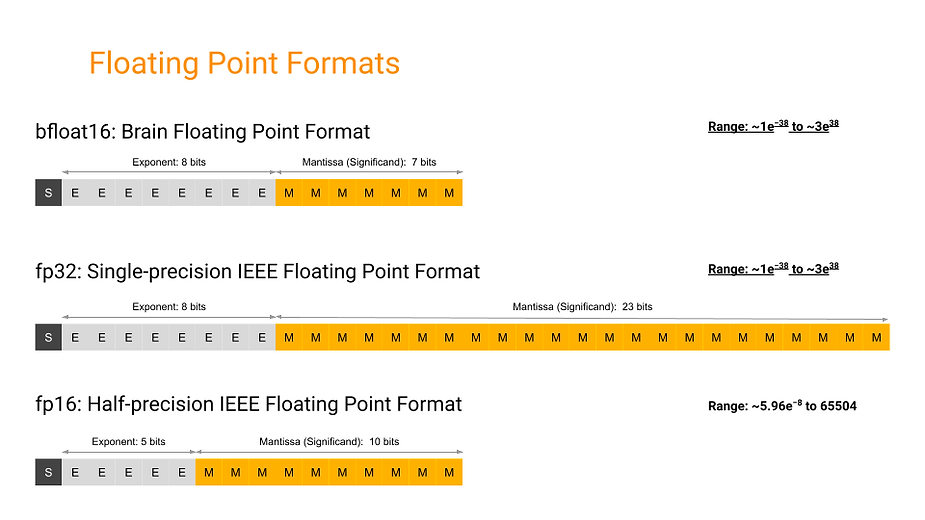
\includegraphics[width=\textwidth]{Images/cap3/quant.png}
    \caption{Formati di rappresentazione dei numeri a virgola mobile \cite{quanttensorops}}
    \label{fig:floatingpoint}
\end{figure}
I tipi di quantizzazione più comuni sono:
\begin{itemize}
    \item \textbf{INT8}: I pesi e le attivazioni vengono rappresentati con 8 bit, riducendo la memoria richiesta per memorizzare i pesi della rete e migliorando la velocità di esecuzione del modello.
    \item \textbf{FP16}: I pesi e le attivazioni contengono numeri a virgola mobile rappresentabili con 16 bit di cui 1 bit per il segno, 5 bit per l'esponente e 10 bit per la mantissa.
    \item \textbf{BF16}: Simile a FP16, ma con più bit dedicati all'esponente, utile per evitare perdite di precisione nelle reti profonde (questa è la quantizzazione usata con i modelli di Hugging Face, vedi Codice \ref{lst:gemma2}).
    \item \textbf{Qn[K S/M/L]}: I pesi e le attivazioni vengono rappresentati con n bit, ma a sua volta esistono varianti a seconda che vengano effettuate o meno delle correzioni sulla perplessità. In quel caso viene aggiunto il suffisso K e una misura di correzione (S/M/L).
\end{itemize}

\subsubsection{Llama3-8B-Q4}
Tornando a Ollama, il modello scelto è stato nuovamente Llama3 da 8B di parametri \cite{llama3ollama}, ma questa volta era disponibile una versione con quantizzazione Q4. Questo ha ridotto significativamente le dimensioni del modello, portandolo a un peso di soli 4.7 GB, rendendolo quindi compatibile con la capacità della VRAM della GPU a disposizione.

Ollama consente di scaricare i modelli disponibili utilizzando il semplice comando \textit{"ollama pull <nome-modello>"}. Successivamente, è possibile avviare una conversazione direttamente da terminale con il comando \textit{"ollama run <nome-modello>"}. Il modello ha fornito risposte in tempi rapidi (circa 1 secondo) e con una buona qualità in diverse lingue, tra cui l'italiano. Pertanto, è stato deciso di utilizzare Ollama per gestire i modelli di NLP all'interno del progetto.

\section{La RAG Chain}
Dopo aver selezionato l'LLM da utilizzare, la decisione successiva è stata quella di integrare la tecnologia RAG nel progetto. Per implementarla, è stato necessario sviluppare l'architettura che gestisse il passaggio dei dati rilevanti all'LLM. Le ricerche hanno condotto rapidamente alla scoperta di LangChain \cite{langchain}.

\subsection{LangChain}
LangChain è un framework di Intelligenza Artificiale che serve a gestire pipeline di elaborazione di modelli di NLP. Esso mette a disposizione numerosi strumenti che possono essere utili per gestire pressoché qualsiasi tipo di azione necessaria all'interno di un progetto di NLP. Questi strumenti spaziano da embedders, vectorstores, retrievers, fino ad arrivare a modelli o agenti.

Il cuore di LangChain è il concetto di "Chain", ovvero una sequenza di azioni che vengono eseguite in ordine. Queste catene possono essere caricate da esempi già pronti, oppure possono essere create da zero sfruttando le risorse messe a disposizione dalle librerie di LangChain.

Per iniziare, è stata creata una RAG Chain di base, in grado di eseguire una ricerca all'interno di un database di documenti e di passare il risultato all'LLM per la generazione di una risposta.

Il primo passo è stato la preparazione dei dati da inserire nel database vettoriale, che è stato possibile grazie ai seguenti elementi:
\begin{itemize}
    \item \textbf{Un Loader di documenti}: Un loader è un oggetto che prende in input dati in un formato specifico e li trasforma nel formato \textit{Document}. Questo formato è usato da LangChain per rappresentare i documenti e contiene due campi principali: \textit{page\textunderscore content}, contenente il testo del documento e \textit{metadata}, formato da un dizionario che contiene informazioni aggiuntive sul documento.
    \item \textbf{Uno Splitter}: Uno splitter è un oggetto che prende in input un Documento e lo divide in Documenti più piccoli. Questo è utile per dividere un testo lungo in paragrafi o frasi.
\end{itemize}
\begin{figure}[!t]
    \centering
    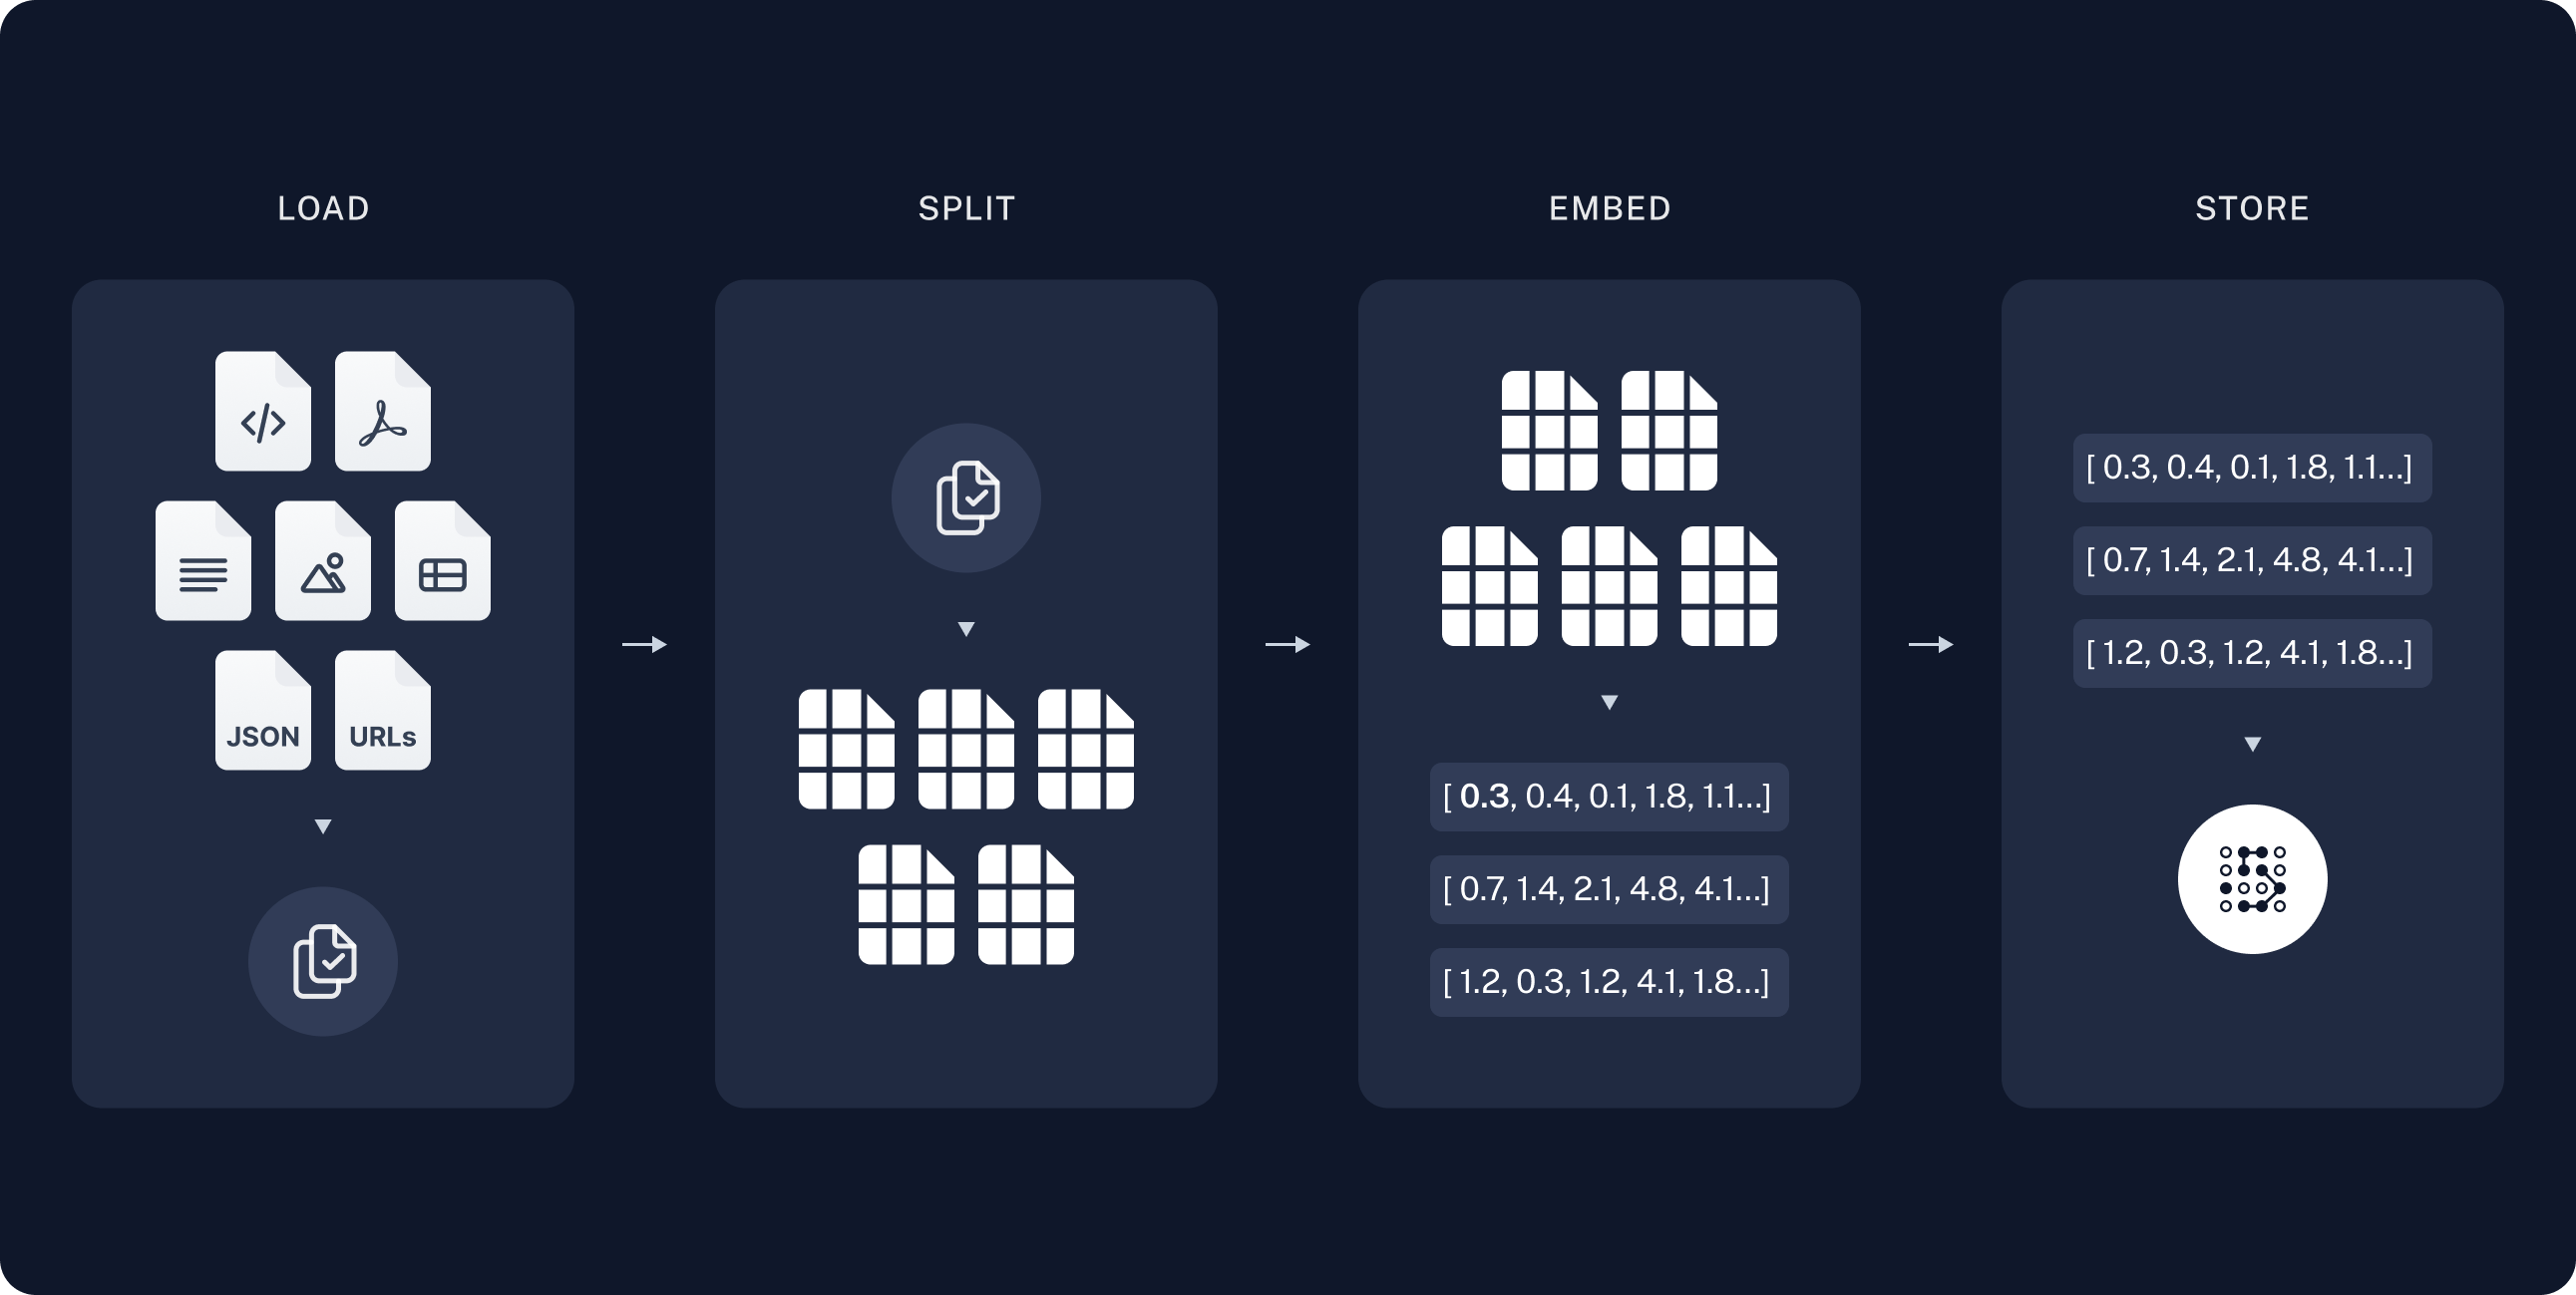
\includegraphics[width=\textwidth]{Images/cap3/rag.png}
    \caption{Indexing dei documenti in un DB Vettoriale \cite{langchainragindexing}}
    \label{fig:indexing}
\end{figure}

Per la prima prova, è stato deciso di utilizzare i documenti tratti dalla pagina Wikipedia di Keanu Reeves \cite{keanureeveswiki}.
\begin{lstlisting}[label=lst:keanusplits, caption={Preparazione degli splits dei documenti di Keanu Reeves}]
from langchain_community.document_loaders import WebBaseLoader
from langchain.text_splitter import RecursiveCharacterTextSplitter
import bs4

loader = WebBaseLoader(*@\textcolor{functionyellow}{(}@*)
    web_paths=(*@\textcolor{keywordpurple}{(}@*)(*@\textcolor{stringbrown}{"https://it.wikipedia.org/wiki/Keanu\_Reeves"}@*),(*@\textcolor{keywordpurple}{)}@*),
    bs_kwargs=(*@\textcolor{classgreen}{dict}@*)(*@\textcolor{keywordpurple}{(}@*)
        parse_only=bs4.SoupStrainer(*@\textcolor{defblue}{(}@*)
            class_=(*@\textcolor{functionyellow}{(}@*)(*@\textcolor{stringbrown}{"mw-content-ltr mw-parser-output"}@*)(*@\textcolor{functionyellow}{)}@*)
        (*@\textcolor{defblue}{)}@*)
    (*@\textcolor{keywordpurple}{)}@*),
    encoding=(*@\textcolor{stringbrown}{"utf-8"}@*)
(*@\textcolor{functionyellow}{)}@*)
splitter = RecursiveCharacterTextSplitter(*@\textcolor{functionyellow}{(}@*)
    chunk_size=(*@\textcolor{numberyellow}{350}@*),
    chunk_overlap=(*@\textcolor{numberyellow}{80}@*)
(*@\textcolor{functionyellow}{)}@*)
loaded = loader.load(*@\textcolor{functionyellow}{()}@*)
splits = splitter.split_documents(*@\textcolor{functionyellow}{(}@*)loaded(*@\textcolor{functionyellow}{)}@*)
\end{lstlisting}
Una volta ottenuti gli splits (o chunks) dei documenti, era necessario vettorizzarli prima di caricarli nel database. Grazie a LangChain queste due operazioni possono essere fatte in un solo passaggio. Per farlo è necessario disporre di due strumenti:
\begin{itemize}
    \item \textbf{Un Embedder}: Un embedder è un oggetto che prende in input un Documento e lo trasforma in un vettore numerico. Questo vettore rappresenta il contenuto del documento in uno spazio vettoriale.
    \item \textbf{Un VectorStore}: Un vectorstore è un oggetto che serve a gestire i vettori generati dagli embedders. Questi vettori vengono memorizzati nel vectorstore e possono essere recuperati in seguito tramite delle ricerche.
\end{itemize}
\begin{lstlisting}[label=lst:keanuload, caption={Caricamento degli splits sul vectorstore}]
from langchain_huggingface import HuggingFaceEmbeddings
from langchain_community.vectorstores import Chroma

model_name = (*@\textcolor{stringbrown}{"sentence-transformers/all-mpnet-base-v2"}@*)
model_kwargs = (*@\textcolor{functionyellow}{\{}@*)"device": "cuda"(*@\textcolor{functionyellow}{\}}@*)
embedder = HuggingFaceEmbeddings(*@\textcolor{functionyellow}{(}@*)
    model_name=model_name,
    model_kwargs=model_kwargs
(*@\textcolor{functionyellow}{)}@*)

vectorstore = Chroma.from_documents(*@\textcolor{functionyellow}{(}@*)
    documents=splits,
    embedding=embedder
(*@\textcolor{functionyellow}{)}@*)
\end{lstlisting}
LangChain offre la possibilità di utilizzare diversi tipi di vectorstores, e il primo che è stato provato è stato \textit{Chroma} \cite{chromadb}, che si è rivelato veloce e preciso. Lo stesso vale per l'embedder: è stato scelto il modello di default offerto da Hugging Face, vale a dire \textit{all-mpnet-base-v2} \cite{mpnet}, sebbene sarebbe stato possibile optare anche per modelli forniti da OllamaEmbeddings o altre librerie. Una volta creato il vectorstore con i vettori dei documenti, è stato possibile effettuare una ricerca all'interno del database. Per questo scopo, è stato necessario implementare un retriever, un oggetto che prende in input una query e restituisce i documenti più rilevanti rispetto alla stessa.
\begin{lstlisting}[label=lst:keanuretriever, caption={Creazione del retriever e primo retrieving}]
retriever = vectorstore.as_retriever(*@\textcolor{functionyellow}{(}@*)
    search_type="similarity", # default
    search_kwargs=(*@\textcolor{keywordpurple}{\{}@*)"k": (*@\textcolor{numberyellow}{2}@*)(*@\textcolor{keywordpurple}{\}}@*) # (*@\textcolor{commentsgreen}{default -> k=4}@*)
(*@\textcolor{functionyellow}{)}@*)
retriever.invoke(*@\textcolor{functionyellow}{(}@*)"Che film ha fatto Keanu Reeves?"(*@\textcolor{functionyellow}{)}@*)
\end{lstlisting}
Il codice in Codice \ref{lst:keanuretriever} crea un retriever e cerca i primi due documenti più simili alla query \textit{"Che film ha fatto Keanu Reeves?"}.

La ricerca dei documenti può essere fatta sia come nell'esempio, ovvero definendo un tipo di retriever a partire dal vectorstore e specificando eventualmente il tipo di ricerca (similarity, mmr, similarity\textunderscore threshold), oppure si può fare direttamente dal vectorstore utilizzando le funzioni di ricerca offerte da esso.

Una volta impostato il retriever, era possibile creare la RAG Chain:
\begin{lstlisting}[label=lst:ragchain, caption={Creazione della RAG Chain}]
from langchain_core.runnables import RunnablePassthrough
from langchain_core.output_parsers import StrOutputParser
from langchain_core.prompts import PromptTemplate

def format_docs(*@\textcolor{functionyellow}{(}@*)docs(*@\textcolor{functionyellow}{)}@*):
    return "\n\n".join(*@\textcolor{functionyellow}{(}@*)doc.page_content for doc in docs(*@\textcolor{functionyellow}{)}@*)

prompt = PromptTemplate.from_template(*@\textcolor{functionyellow}{(}@*)RAG_PROMPT(*@\textcolor{functionyellow}{)}@*)

rag_chain = (*@\textcolor{functionyellow}{(}@*)
    (*@\textcolor{keywordpurple}{\{}@*)
        "context": retriever | format_docs,
        "question": RunnablePassthrough(*@\textcolor{defblue}{()}@*)
    (*@\textcolor{keywordpurple}{\}}@*)
    | prompt
    | llm
    | StrOutputParser(*@\textcolor{keywordpurple}{()}@*)
(*@\textcolor{functionyellow}{)}@*)

rag_chain.invoke(*@\textcolor{functionyellow}{(}@*)"Che film ha fatto Keanu Reeves?"(*@\textcolor{functionyellow}{)}@*)
\end{lstlisting}
Questo basta per creare una RAG Chain che permetta di effettuare ricerche all'interno di un database di documenti e passare il risultato all'LLM per la generazione di una risposta. Da notare il prompt utilizzato, che è stato definito in precedenza nel Codice \ref{lst:prompt} e che permette di formattare l'input in modo che sia comprensibile dall'LLM. In più è stata definita una funzione \textit{format\textunderscore docs()} che permette di formattare i documenti in modo da passare solo il contenuto del documento all'LLM.

\subsection{I primi problemi}
Eseguendo lo script appena descritto, il risultato ottenuto è stato il seguente:
\begin{center}
    \textit{"Keanu Reeves è un attore che ha interpretato ruoli in diversi film, ad esempio Spalle Larghe (Youngblood) e Il fantastico mondo dei giocattoli (Babes in Toyland)."}
\end{center}
L'output è stato generato in circa 3 minuti, è corretto, ma non è dei migliori poiché avrebbe potuto includere più informazioni. Tentando nuovamente, ma senza includere il passaggio in cui il retriever cerca i documenti più simili alla query (quindi passando l'input direttamente all'LLM), l'output generato è stato il seguente:
\begin{center}
    \textit{"Keanu Reeves è un attore canadese naturalizzato statunitense. Ha recitato in molti film di successo, tra cui Speed, Matrix e John Wick."}
\end{center}
Questa volta esso è stato generato nella metà del tempo e nonostante contenga informazioni meno dettagliate, ha risposto includendo informazioni molto più varie e di maggior rilevanza. Questo output però si basa solo sulle conoscenze del modello e non su documenti caricati.

Il problema principale è che il retriever non è stato in grado di trovare i documenti più rilevanti alla query, e questo è dovuto al fatto che i documenti caricati nel database non erano sufficientemente informativi. Si è quindi deciso di testare domande più semplici, che richiedessero meno informazioni. L'input scelto è stato: \textit{"Dimmi quando e dove è nato Keanu Reeves"}, e l'output generato è stato il seguente:
\begin{center}
    \textit{"Keanu Reeves è nato nel 1964 a Beirut, in Libano, il giorno del suo compleanno."}
\end{center}
L'output generato è corretto, in quanto Keanu Reeves è effettivamente nato a Beirut, Libano, nel 1964. Tuttavia, peccava di precisione e consistenza. Si ipotizzò che il problema fosse legato al fatto che l'input ricevuto dal retriever fosse esattamente la query dell'utente, e che questo potesse non essere sufficiente per identificare i documenti più rilevanti. Inoltre, la formattazione dei dati caricati dalla pagina Wikipedia di Keanu Reeves non era ottimale, il che potrebbe aver influito sulla qualità dei risultati.

\subsection{Il DB Maker}
\label{sec:dbmaker}
Per mitigare il problema, è stata creata una struttura con il compito di gestire l'intero processo di indicizzazione dei dati grezzi. Questo sistema, evoluto nel DB Maker, prende in input una lista di oggetti di tipo \textit{Data}, ciascuno contenente tutte le informazioni necessarie per accedere ai dati che rappresentano. Tra queste informazioni, è presente un campo di tipo \textit{DataType}, che indica il tipo di dati contenuti nell'oggetto. A seconda del tipo di dato, viene utilizzato un tipo di loader differente. I dati supportati dal DB Maker sono: Web, File Testuali, Dataframe e PDF. Questi possono essere caricati singolarmente o specificando una directory, lasciando al DB Maker il compito di discernere i vari tipi di dati.

Una volta che il Maker ha ottenuto tutte le informazioni necessarie, avvia un test per verificare che i dati che si intende caricare siano esistenti e correttamente accessibili. In caso positivo, inizia il processo di caricamento e suddivisione dei dati. Una volta ottenuti gli splits, i dati vengono vettorizzati e caricati nel vectorstore. Inizialmente, è stato scelto Chroma come vectorstore, ma a causa di problemi riscontrati durante il tentativo di caricare dati di dimensioni maggiori, sono state effettuate alcune prove con altri strumenti.

È stato provato il vectorstore \textit{QDrant} \cite{qdrant}, che, nonostante la sua eccezionale velocità sia in fase di inserimento dei dati che in fase di recupero, ha mostrato imprecisione nei risultati. Il migliore, alla fine, si è rivelato essere \textit{FAISS} \cite{faiss,douze2024faisslibrary}, che si è dimostrato sia veloce che preciso.
\begin{lstlisting}[label=lst:dbmaker, caption={Implementazione del DB Maker}]
from data_manager import Data, Splitter
from langchain_community.vectorstores import FAISS
from tqdm import tqdm

class DBMaker(*@\textcolor{functionyellow}{()}@*):
    def __init__(*@\textcolor{functionyellow}{(}@*)self, config: (*@\textcolor{classgreen}{dict}@*), vectorstore: FAISS(*@\textcolor{functionyellow}{)}@*):
        self.config = config
        self.vectorstore = vectorstore
    
    def make(*@\textcolor{functionyellow}{(}@*)self, data: (*@\textcolor{classgreen}{list}@*)(*@\textcolor{keywordpurple}{[}@*)Data(*@\textcolor{keywordpurple}{]}@*)(*@\textcolor{functionyellow}{)}@*):
        splitter = Splitter(*@\textcolor{functionyellow}{(}@*)self.config(*@\textcolor{keywordpurple}{[}@*)"paths"(*@\textcolor{keywordpurple}{]}@*)(*@\textcolor{keywordpurple}{[}@*)"data"(*@\textcolor{keywordpurple}{]}@*)(*@\textcolor{functionyellow}{)}@*)
        docs = splitter.create_chunks(*@\textcolor{functionyellow}{(}@*)data(*@\textcolor{functionyellow}{)}@*)
        batches = self.batch(*@\textcolor{functionyellow}{(}@*)docs(*@\textcolor{functionyellow}{)}@*)
        for (*@\textcolor{basicblue}{batch}@*) in tqdm(*@\textcolor{functionyellow}{(}@*)
            batches,
            desc="Caricamento documenti(*@\textcolor{stringbrown}{...}@*)"
        (*@\textcolor{functionyellow}{)}@*):
            self.vectorstore.add_documents(*@\textcolor{functionyellow}{(}@*)(*@\textcolor{basicblue}{batch}@*)(*@\textcolor{functionyellow}{)}@*)
        self.vectorstore.save_local(*@\textcolor{functionyellow}{(}@*)
            self.config(*@\textcolor{keywordpurple}{[}@*)"paths"(*@\textcolor{keywordpurple}{]}@*)(*@\textcolor{keywordpurple}{[}@*)"db"(*@\textcolor{keywordpurple}{]}@*)
        (*@\textcolor{functionyellow}{)}@*)
    
    def batch(*@\textcolor{functionyellow}{(}@*)self, chunks, n_max=(*@\textcolor{numberyellow}{10000}@*)(*@\textcolor{functionyellow}{)}@*):
        batches = (*@\textcolor{functionyellow}{[]}@*)
        current_batch = (*@\textcolor{functionyellow}{[]}@*)
        count = (*@\textcolor{numberyellow}{0}@*)

        for c in chunks:
            chunk_length = len(*@\textcolor{functionyellow}{(}@*)c.page_content(*@\textcolor{functionyellow}{)}@*)
            
            if count + chunk_length >= n_max:
                batches.append(*@\textcolor{functionyellow}{(}@*)current_batch(*@\textcolor{functionyellow}{)}@*)
                current_batch = (*@\textcolor{functionyellow}{[}@*)c(*@\textcolor{functionyellow}{]}@*)
                count = chunk_length
            else:
                current_batch.append(*@\textcolor{functionyellow}{(}@*)c(*@\textcolor{functionyellow}{)}@*)
                count += chunk_length

        if current_batch:
            batches.append(*@\textcolor{functionyellow}{(}@*)current_batch(*@\textcolor{functionyellow}{)}@*)
        
        return batches
\end{lstlisting}
Il Codice \ref{lst:dbmaker} è l'implementazione del DB Maker, si noti che i documenti vengono caricati in batch di dimensioni massime di 10000 caratteri. Questo è stato fatto per evitare che la memoria di sistema si riempisse troppo velocemente.
Lo splitter invece è implementato in modo tale da prendere in input i dati grezzi e passarli al loro loader corrispondente. A quel punto effettua lo splitting dei documenti e li restituisce tutti assieme al DB Maker all'interno di una lista di oggetti di tipo Document.
\begin{lstlisting}[label=lst:loaddb, caption={Procedura di caricamento con DB Maker}]
from langchain_community.docstore import InMemoryDocstore
from langchain_community.vectorstores import FAISS
from langchain_huggingface import HuggingFaceEmbeddings

from data_manager import DataList
from (*@\textcolor{classgreen}{db\_maker}@*) import DBMaker
from utilities import load_config
from dotenv import load_dotenv, find_dotenv
import faiss
import torch
 
config = load_config(*@\textcolor{functionyellow}{()}@*)
load_dotenv(*@\textcolor{functionyellow}{(}@*)find_dotenv(*@\textcolor{keywordpurple}{()}@*)(*@\textcolor{functionyellow}{)}@*)

data_list = DataList(*@\textcolor{functionyellow}{(}@*)config(*@\textcolor{functionyellow}{)}@*)
data_list.add_dir(*@\textcolor{functionyellow}{(}@*)
    path="txts_parags/",
    chunk_size=(*@\textcolor{numberyellow}{1000}@*),
    chunk_overlap=(*@\textcolor{numberyellow}{0}@*)
(*@\textcolor{functionyellow}{)}@*)
data_list.add(*@\textcolor{functionyellow}{(}@*)path="link(*@\textcolor{stringbrown}{.}@*)txt"(*@\textcolor{functionyellow}{)}@*)

if not data_list.test(*@\textcolor{functionyellow}{()}@*):
    return
data = data_list.get_data(*@\textcolor{functionyellow}{()}@*)

model_name = config(*@\textcolor{functionyellow}{[}@*)"embedder"(*@\textcolor{functionyellow}{]}@*)
device = "cuda" if torch.cuda.is_available(*@\textcolor{functionyellow}{()}@*) else "cpu"
model_kwargs = (*@\textcolor{functionyellow}{\{}@*)"device": device(*@\textcolor{functionyellow}{\}}@*)

embedder = HuggingFaceEmbeddings(*@\textcolor{functionyellow}{(}@*)
    model_name=model_name,
    model_kwargs=model_kwargs
(*@\textcolor{functionyellow}{)}@*)

index = faiss.IndexFlatL2(*@\textcolor{functionyellow}{(}@*)
    len(*@\textcolor{keywordpurple}{(}@*)embedder.embed_query(*@\textcolor{defblue}{(}@*)"index"(*@\textcolor{defblue}{)}@*)(*@\textcolor{keywordpurple}{)}@*)
(*@\textcolor{functionyellow}{)}@*)

vectorstore = FAISS(*@\textcolor{functionyellow}{(}@*)
    embedding_function=embedder,
    index=index,
    (*@\textcolor{basicblue}{docstore}@*)=InMemoryDocstore(*@\textcolor{keywordpurple}{()}@*),
    index_to_docstore_id=(*@\textcolor{keywordpurple}{\{\}}@*)
(*@\textcolor{functionyellow}{)}@*)

db_maker = DBMaker(*@\textcolor{functionyellow}{(}@*)config, vectorstore(*@\textcolor{functionyellow}{)}@*)
db_maker.make(*@\textcolor{functionyellow}{(}@*)data(*@\textcolor{functionyellow}{)}@*)
\end{lstlisting}
In questo modo, è possibile creare un database vettoriale con i documenti di interesse e salvarlo localmente. Una volta creato il database, esso può essere utilizzato ripetutamente per eseguire ricerche nei documenti, senza la necessità di ricaricarli ogni volta.

Come illustrato all'inizio del Codice \ref{lst:loaddb}, i dati vengono caricati all'interno di un oggetto di tipo \textit{DataList}. Questi dati provengono da una directory, tranne che per un singolo file contenente alcuni link, che viene caricato singolarmente. Dopo che i dati sono stati inseriti, vengono sottoposti a un test per verificare che siano corretti e accessibili. Se il test ha esito positivo, i dati possono essere caricati nel vectorstore.

Per l'embedder, viene utilizzato lo stesso modello degli esempi precedenti (vedi Codice \ref{lst:keanuload}). Per quanto riguarda il vectorstore, si utilizza FAISS, che richiede (oltre ai documenti e all'embedder) un indice e un docstore. L'indice è un oggetto di tipo \textit{faiss.IndexFlatL2}, un indice piatto con distanza euclidea che si occupa di memorizzare i vettori veri e propri e gestire la loro ricerca. Il docstore è un oggetto di tipo \textit{InMemoryDocstore}, che serve a memorizzare i dati dei documenti in memoria. Quando viene trovato un determinato vettore, è possibile accedere al suo ID e, di conseguenza, al documento corrispondente nel docstore  (tramite l'indice \textit{index\textunderscore to\textunderscore docstore\textunderscore id}). In questo modo, è possibile recuperare i dati del documento associato al vettore trovato.